In this section, I will demonstrate that every \textsc{EviL} model
corresponds to some highly structured Kripke model, with a minor
modification on the standard definition.  However, it will turn out
that this correspondence is one way - the class of Kripke models for
which \textsc{EviL} is strongly complete do not, in general,
possess corresponding \textsc{EviL} models.

However, to elucidate my intuition for understanding \textsc{EviL} models as
Kripke models, I would like to return to the visualization technique for
\textsc{EviL} models I introduced in \S(FIXME).  This involved, roughly,
thinking of the \textsc{EviL} models as \emph{posets} with arrows,
as I first presented in Fig. \ref{fig:example1}.  I have given
additional examples in Figs. \ref{fig:example2} and
\ref{fig:example3}.  
In all of these depictions, the implicit relational structure of \textsc{EviL} models is given
visual expression.  So it seems only natural to me that this graphically perceived structure
could also find formal expression.
\begin{figure}[ht]
\centering
\subfigure[A fairly simple example]{
  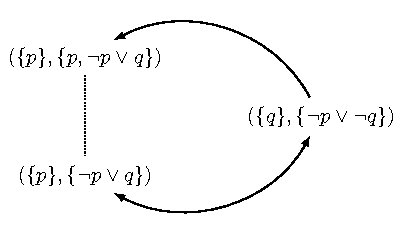
\includegraphics[]{evil_pictures/first_fig.pdf}
%\caption{A fairly simple example}
\label{fig:example2}
}
\subfigure[A more complex example]{
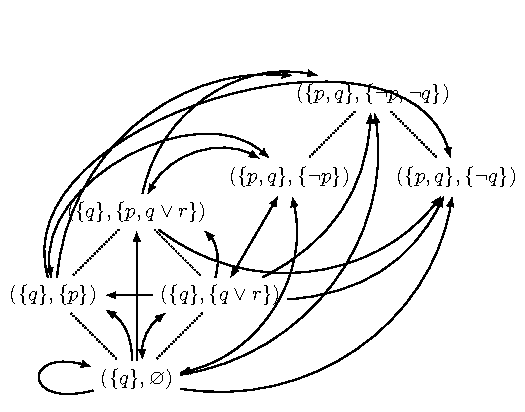
\includegraphics[]{evil_pictures/second_fig.pdf}
\label{fig:example3}
}
\caption{\textsc{EviL} model visualizations}
\end{figure}

Following the modified semantics provided in \S\ref{multi-agent}, the
developments this section will assume multiple agents.
\begin{definition}
  Let $\Phi$ be a set of letters and let $\mathcal{A}$ be a set of agents. \
  A \textbf{Kripke structure} is a state transition system $\mathbb{M}=\langle W^{\mathbb{M}}, R^{\mathbb{M}},
  \sqsubseteq^{\mathbb{M}}, \sqsupseteq^{\mathbb{M}}, V^{\mathbb{M}},
  P^{\mathbb{M}}_{\circlearrowleft} \rangle$ where\footnote{Where
    the context is clear, I shall drop $\mathbb{M}$ from the
    superscripts I am employing.}:
  \begin{itemizedot}
    \item $W^{\mathbb{M}}$ is a set of worlds    
    \item $R^{\mathbb{M}} : \mathcal{A} \rightarrow \powerset (W \times W)$, $\sqsubseteq^{\mathbb{M}} : \mathcal{A} \rightarrow \powerset (W \times W)$, and $\sqsupseteq^{\mathbb{M}} : \mathcal{A} \rightarrow \powerset (W \times W)$ are
    $\mathcal{A}$-indexed sets of relations\footnote{I will abbreviate
      $R(X)$, $\sqsubseteq(X)$ and $\sqsupseteq(X)$ as $R(X)$,
      $\sqsubseteq(X)$ and $\sqsupseteq(X)$ as $R_X$, $\sqsubseteq_X$
      and $\sqsupseteq_X$ respectively.}
    \item $V : \Phi \rightarrow \powerset (W)$ is a predicate letter valuation
    \item $P_{\circlearrowleft} : \mathcal{A} \rightarrow \powerset
      (W)$ are sets of worlds indexed by agents
  \end{itemizedot}
  Let $\mathcal{K}_{\Phi, \mathcal{A}, I}$ denote the class of Kripke structures for letters $\Phi$, agents $\mathcal{A}$, and where $W \subseteq I$.
\end{definition}
Kripke semantics given by $(\Vdash) : \mathcal{K}_{\Phi, \mathcal{A}, I} \to I
\rightarrow \text{\tmtextsf{bool}}$ for these models are defined recursively
as usual, granted the exceptional behavior of $P_{\circlearrowleft}$.
\begin{definition}
  Let $\mathbbm{M}$ be in the class $\mathcal{K}_{\Phi, \mathcal{A}, I}$
  \begin{eqnarray*}
    \mathbbm{M}, w \Vdash p & \Longleftrightarrow & w \in V^{\mathbbm{M}}
    (p)\\
    \mathbbm{M}, w \Vdash \phi \rightarrow \psi & \Longleftrightarrow &
    \mathbbm{M}, w \Vdash \phi \text{ implies } \mathbbm{M}, w \Vdash \psi\\
    \mathbbm{M}, w \Vdash \bot & \Longleftrightarrow & \text{False}\\
    \mathbbm{M}, w \Vdash \Box_X \phi & \Longleftrightarrow & \forall v \in
    W^{\mathbbm{M}} . w R^{\mathbbm{M}}_X v \text{ implies } \mathbbm{M}, v
    \Vdash \phi\\
    \mathbbm{M}, w \Vdash \boxminus_X \phi & \Longleftrightarrow & \forall v
    \in W^{\mathbbm{M}} . w \sqsupseteq^{\mathbbm{M}}_X v \text{ implies }
    \mathbbm{M}, v \Vdash \phi\\
    \mathbbm{M}, w \Vdash \boxplus_X \phi & \Longleftrightarrow & \forall v
    \in W^{\mathbbm{M}} . w \sqsubseteq^{\mathbbm{M}}_X v \text{ implies }
    \mathbbm{M}, v \Vdash \phi\\
    \mathbbm{M}, w \Vdash \circlearrowleft_X & \Longleftrightarrow & w \in
    P_{\circlearrowleft}^{\mathbbm{M}} (X)
  \end{eqnarray*}
\end{definition}
Kripke structures can be observe to have a lot less structure than
\tmtextsc{EviL} models.  However, \tmtextsc{EviL} models can be understood as
Kripke structures in disguise.  To illustrate this, observe the following
lemma:
\begin{definition}[$\mho^\Omega$ Translation]
Let $\Omega$ be an \tmtextsc{EviL} model.  Define
  $\mho^{\Omega} \assign \langle \Omega, R^{\Omega},
  \sqsubseteq^{\Omega}, \sqsupseteq^{\Omega}, V^{\Omega},
  P_{\circlearrowleft}^{\Omega} \rangle$, where
  \[ \begin{array}{llll}
       \bullet & \text{$(a, A) R^{\Omega}_X (b, B) \Longleftrightarrow \forall
       \psi \in A_X .b \models \psi$} & \bullet & (a, A)
       \sqsubseteq^{\Omega}_X (b, B) \Longleftrightarrow a = b \text{ and }
       A_X \subseteq B_X\\
       \bullet & (a, A) \sqsupseteq^{\Omega}_X (b, B) \Longleftrightarrow a =
       b \text{ and } A_X \supseteq B_X & \bullet & (a, A) \in
       P_{\circlearrowleft}^{\Omega} (X) \Longleftrightarrow \forall \psi \in
       A_X .a \models \psi
     \end{array} \]
\end{definition}
\begin{lemma}
  \label{tranlemma1} For all $\Omega$ and all $(a, A) \in \Omega$,  $\Omega, (a, A) \VDash
  \phi$ if and only if $\mho^{\Omega}, (a, A) \Vdash \phi$
\end{lemma}
\begin{proof}
  This follows from a straightforward induction on $\phi$.
\end{proof}
The following summarizes the structural properties of
\tmtextsc{EviL} models, when transformed into Kripke structures:
\begin{proposition}
  For any \textsc{EviL} model $\Omega$,  $\mho^{\Omega}$ has the following
  properties{\footnote{Note that in this we have that $\{w,v\} \subseteq \powerset \Phi
      \times \powerset \mathcal{L}_0$ in the subsequent discussion}}:
  \begin{myRoman}
    \item\label{pI} $\sqsupseteq^{\Omega}_X$ is reflexive
    \item $\sqsupseteq^{\Omega}_X$ is transitive 
    \item \label{pantisym}$\sqsupseteq^{\Omega}_X$ is anti-symmetric
    \item $w \sqsupseteq^{\Omega}_X v$ if and only if $v
    \sqsubseteq^{\Omega}_X w$
    \item If $w \sqsubseteq^{\Omega}_X v$ then $w \in V (p)$ if and only if $v
    \in V (p)$
    \item \label{pV}$R^{\Omega}_X \circ \sqsubseteq^{\Omega}_X \subseteq
    R^{\Omega}_X \subseteq R^{\Omega}_X \circ \sqsupseteq^{\Omega}_X$
    \item $\sqsubseteq^{\Omega}_Y \circ R^{\Omega}_X = R^{\Omega}_X =
    \sqsupseteq^{\Omega}_Y \circ R^{\Omega}_X$
    \item\label{propVII} $w \in P_{\circlearrowleft}^{\Omega} (X)$ if and only if $w
    R^{\Omega}_X w$
  \end{myRoman}
\end{proposition}
\begin{proof}
  Everything except \ref{pV} follows directly from the definitions - so I shall only
  demonstrate $R^{\Omega}_X \subseteq R^{\Omega}_X \circ
  \sqsupseteq^{\Omega}_X$.
  
  Suppose that $(a, A) R^{\Omega}_X (b, B)$, then evidently $\forall \psi \in
  A_X .b \models \psi$. 
  Now assume that $(a, A) \sqsupseteq_X^{\Omega} (c,
  C)$.  Then we know that $A_X \supseteq C_X$.
  But then $\forall \psi \in
  C_X .b \models \psi$, so $(c, C) R^{\Omega}_X (b, B)$, which
  suffices to show the claim.
\end{proof}

\begin{definition}
A Kripke structure is called \tmtextsc{EviL} if it makes true the
  above properties \ref{pI} through \ref{pVII} (with the exception of \ref{pantisym}, which is optional).
\end{definition}

These properties are definitive - as we shall demonstrate, \tmtextsc{EviL} is
sound and weakly complete for \tmtextsc{EviL} models.

The Kripke semantics also serve to \ provide proper intuition behind
\tmtextsc{EviL} models. \ I think of the defined relations given as follows:
\begin{itemizedot}
  \item If $x R^{\Omega}_X y$, then at world $x$ the agent $X$ can imagine $y$
  is true, since $y$ is compatible with what the agent believes 
  \item If $x \sqsubseteq^{\Omega}_X y$, then at world $x$, agent $X$'s
  assumptions (or the experiences they are taking under consideration) are
  contained in her evidence at $y$
\end{itemizedot}
Given this perspective, the proof of \ref{pV} can be understood in the
following way - if the agent assumes fewer things, more things are imaginable,
since it's easier for a world to be incompatible with an agent's evidence.

In fact, in light of Theorem \ref{theorem-theorem}, the above follows
from an underlying, order theoretic relationship present in model theory.  For a given
Kripke structure $\mathbbm{M}$, define two operators $Mod^{\mathbbm{M}}
: \powerset  \mathcal{L} (\Phi, \mathcal{A}) \rightarrow \powerset
(W^{\mathbbm{M}})$ and $Th^{\mathbbm{M}} : \powerset
(W^{\mathbbm{M}}) \rightarrow \powerset \mathcal{L} (\Phi, \mathcal{A})$
\begin{align*}
  Mod^{{\mathbbm{M}}}({\Delta}) &
  =\{x{\in}W{\ }|{\ }{\forall}{\psi}{\in}{\Delta}.
  {\mathbbm{M}},x{\Vdash}{\psi}\}\\
  Th^{{\mathbbm{M}}}({\nabla}) & =\{{\psi}{\in}\mathcal{L}({\Phi},
  \mathcal{A}){\ }|{\ }{\forall}x{\in}{\nabla}.
  {\mathbbm{M}},x{\Vdash}{\psi}\}
\end{align*}
We then have, for any $\Delta \in \powerset  \mathcal{L}
(\Phi, \mathcal{A})$ and $\nabla \in \powerset (W^{\mathbbm{M}})$:
\[ \nabla \subseteq Mod^{\mathbbm{M}} (\Delta) \text{ if and only if }
   \Delta \subseteq Th^{\mathbbm{M}} (\nabla) \]
$\ldots$hence we these two operations form what is refered an
\emph{antitone Galois connection}, between the lattice $\powerset
(W^{\mathbbm{M}})$ and the lattice $\powerset \mathcal{L} (\Phi,
\mathcal{A})$. It follows from the theory of Galois connections
\citep[][chapter 3]{roman_lattices_2008} that
the following two properties:
\begin{itemizedot}
  \item If $\nabla \supseteq \nabla'$ then $Th^{\mathbbm{M}} (\nabla)
  \subseteq Th^{\mathbbm{M}} (\nabla')$
  \item If $\Delta \supseteq \Delta'$ then $Mod^{\mathbbm{M}} (\Delta)
  \subseteq Mod^{\mathbbm{M}} (\Delta')$
\end{itemizedot}
We can see that (\ref{pV}) follows from the second of these two properties. \
To see this, assume that $(a, A) \sqsupseteq_X^{\Omega} (b, B)$, hence $A_X
\supseteq B_X$ and thus $Mod^{\Omega} (A_X) \subseteq
Mod^{\Omega} (B_X)$. \ But it follows from semantics of \tmtextsc{EviL}
we have that $(c, C) \in Mod^{\Omega} (A_X)$ if and only if $(a, A)
R^{\Omega}_X (c, C)$, and likewise for $B_X$. \ Hence if $(a, A) R^{\Omega}_X
(c, C)$ then $(b, B) R^{\Omega}_X (c, C)$.

%%% Local Variables: 
%%% mode: latex
%%% TeX-master: "evil_philosophy"
%%% End: 
